% Options for packages loaded elsewhere
\PassOptionsToPackage{unicode}{hyperref}
\PassOptionsToPackage{hyphens}{url}
%
\documentclass[
]{article}
\usepackage{lmodern}
\usepackage{amssymb,amsmath}
\usepackage{ifxetex,ifluatex}
\ifnum 0\ifxetex 1\fi\ifluatex 1\fi=0 % if pdftex
  \usepackage[T1]{fontenc}
  \usepackage[utf8]{inputenc}
  \usepackage{textcomp} % provide euro and other symbols
\else % if luatex or xetex
  \usepackage{unicode-math}
  \defaultfontfeatures{Scale=MatchLowercase}
  \defaultfontfeatures[\rmfamily]{Ligatures=TeX,Scale=1}
\fi
% Use upquote if available, for straight quotes in verbatim environments
\IfFileExists{upquote.sty}{\usepackage{upquote}}{}
\IfFileExists{microtype.sty}{% use microtype if available
  \usepackage[]{microtype}
  \UseMicrotypeSet[protrusion]{basicmath} % disable protrusion for tt fonts
}{}
\makeatletter
\@ifundefined{KOMAClassName}{% if non-KOMA class
  \IfFileExists{parskip.sty}{%
    \usepackage{parskip}
  }{% else
    \setlength{\parindent}{0pt}
    \setlength{\parskip}{6pt plus 2pt minus 1pt}}
}{% if KOMA class
  \KOMAoptions{parskip=half}}
\makeatother
\usepackage{xcolor}
\IfFileExists{xurl.sty}{\usepackage{xurl}}{} % add URL line breaks if available
\IfFileExists{bookmark.sty}{\usepackage{bookmark}}{\usepackage{hyperref}}
\hypersetup{
  pdftitle={Specificity and Methylation sensitivity analysis of CTCF(F1-F9)},
  pdfauthor={Zheng Zuo},
  hidelinks,
  pdfcreator={LaTeX via pandoc}}
\urlstyle{same} % disable monospaced font for URLs
\usepackage[margin=1in]{geometry}
\usepackage{color}
\usepackage{fancyvrb}
\newcommand{\VerbBar}{|}
\newcommand{\VERB}{\Verb[commandchars=\\\{\}]}
\DefineVerbatimEnvironment{Highlighting}{Verbatim}{commandchars=\\\{\}}
% Add ',fontsize=\small' for more characters per line
\usepackage{framed}
\definecolor{shadecolor}{RGB}{248,248,248}
\newenvironment{Shaded}{\begin{snugshade}}{\end{snugshade}}
\newcommand{\AlertTok}[1]{\textcolor[rgb]{0.94,0.16,0.16}{#1}}
\newcommand{\AnnotationTok}[1]{\textcolor[rgb]{0.56,0.35,0.01}{\textbf{\textit{#1}}}}
\newcommand{\AttributeTok}[1]{\textcolor[rgb]{0.77,0.63,0.00}{#1}}
\newcommand{\BaseNTok}[1]{\textcolor[rgb]{0.00,0.00,0.81}{#1}}
\newcommand{\BuiltInTok}[1]{#1}
\newcommand{\CharTok}[1]{\textcolor[rgb]{0.31,0.60,0.02}{#1}}
\newcommand{\CommentTok}[1]{\textcolor[rgb]{0.56,0.35,0.01}{\textit{#1}}}
\newcommand{\CommentVarTok}[1]{\textcolor[rgb]{0.56,0.35,0.01}{\textbf{\textit{#1}}}}
\newcommand{\ConstantTok}[1]{\textcolor[rgb]{0.00,0.00,0.00}{#1}}
\newcommand{\ControlFlowTok}[1]{\textcolor[rgb]{0.13,0.29,0.53}{\textbf{#1}}}
\newcommand{\DataTypeTok}[1]{\textcolor[rgb]{0.13,0.29,0.53}{#1}}
\newcommand{\DecValTok}[1]{\textcolor[rgb]{0.00,0.00,0.81}{#1}}
\newcommand{\DocumentationTok}[1]{\textcolor[rgb]{0.56,0.35,0.01}{\textbf{\textit{#1}}}}
\newcommand{\ErrorTok}[1]{\textcolor[rgb]{0.64,0.00,0.00}{\textbf{#1}}}
\newcommand{\ExtensionTok}[1]{#1}
\newcommand{\FloatTok}[1]{\textcolor[rgb]{0.00,0.00,0.81}{#1}}
\newcommand{\FunctionTok}[1]{\textcolor[rgb]{0.00,0.00,0.00}{#1}}
\newcommand{\ImportTok}[1]{#1}
\newcommand{\InformationTok}[1]{\textcolor[rgb]{0.56,0.35,0.01}{\textbf{\textit{#1}}}}
\newcommand{\KeywordTok}[1]{\textcolor[rgb]{0.13,0.29,0.53}{\textbf{#1}}}
\newcommand{\NormalTok}[1]{#1}
\newcommand{\OperatorTok}[1]{\textcolor[rgb]{0.81,0.36,0.00}{\textbf{#1}}}
\newcommand{\OtherTok}[1]{\textcolor[rgb]{0.56,0.35,0.01}{#1}}
\newcommand{\PreprocessorTok}[1]{\textcolor[rgb]{0.56,0.35,0.01}{\textit{#1}}}
\newcommand{\RegionMarkerTok}[1]{#1}
\newcommand{\SpecialCharTok}[1]{\textcolor[rgb]{0.00,0.00,0.00}{#1}}
\newcommand{\SpecialStringTok}[1]{\textcolor[rgb]{0.31,0.60,0.02}{#1}}
\newcommand{\StringTok}[1]{\textcolor[rgb]{0.31,0.60,0.02}{#1}}
\newcommand{\VariableTok}[1]{\textcolor[rgb]{0.00,0.00,0.00}{#1}}
\newcommand{\VerbatimStringTok}[1]{\textcolor[rgb]{0.31,0.60,0.02}{#1}}
\newcommand{\WarningTok}[1]{\textcolor[rgb]{0.56,0.35,0.01}{\textbf{\textit{#1}}}}
\usepackage{graphicx}
\makeatletter
\def\maxwidth{\ifdim\Gin@nat@width>\linewidth\linewidth\else\Gin@nat@width\fi}
\def\maxheight{\ifdim\Gin@nat@height>\textheight\textheight\else\Gin@nat@height\fi}
\makeatother
% Scale images if necessary, so that they will not overflow the page
% margins by default, and it is still possible to overwrite the defaults
% using explicit options in \includegraphics[width, height, ...]{}
\setkeys{Gin}{width=\maxwidth,height=\maxheight,keepaspectratio}
% Set default figure placement to htbp
\makeatletter
\def\fps@figure{htbp}
\makeatother
\setlength{\emergencystretch}{3em} % prevent overfull lines
\providecommand{\tightlist}{%
  \setlength{\itemsep}{0pt}\setlength{\parskip}{0pt}}
\setcounter{secnumdepth}{-\maxdimen} % remove section numbering

\title{Specificity and Methylation sensitivity analysis of CTCF(F1-F9)}
\author{Zheng Zuo}
\date{Sep 12, 2020}

\begin{document}
\maketitle

{
\setcounter{tocdepth}{2}
\tableofcontents
}
\hypertarget{background-and-introduction}{%
\subsection{Background and
Introduction}\label{background-and-introduction}}

The CTCF protein, consisting of 11 tandem C2H2-type zinc fingers, is
known to be critical insultor for genome architecture in mammals. Its
finger 3 to 7 has been shown to recognize underlying reference sequence
and motif strongly. Also It was known that CTCF processes some
methylation sensitivity, i.e., when some CpG dinucleotide gets
methylated within the binding site, the affinity of CTCF to the
methylated sites gets compromised. To systematically investigate the
specificity and methylation sensitivity of mouse CTCF protein, I
designed and synthesized the following dsDNA libraries, covering every
single and adjacent double variants of the core binding sites recognized
by F3-F7. Position 19 serves as the barcode position to indicate
wheather each sequence is treated by M.SssI methylated beforehand or not
(For M.SssI treatment, only CpG dinucleotide can get methylated).

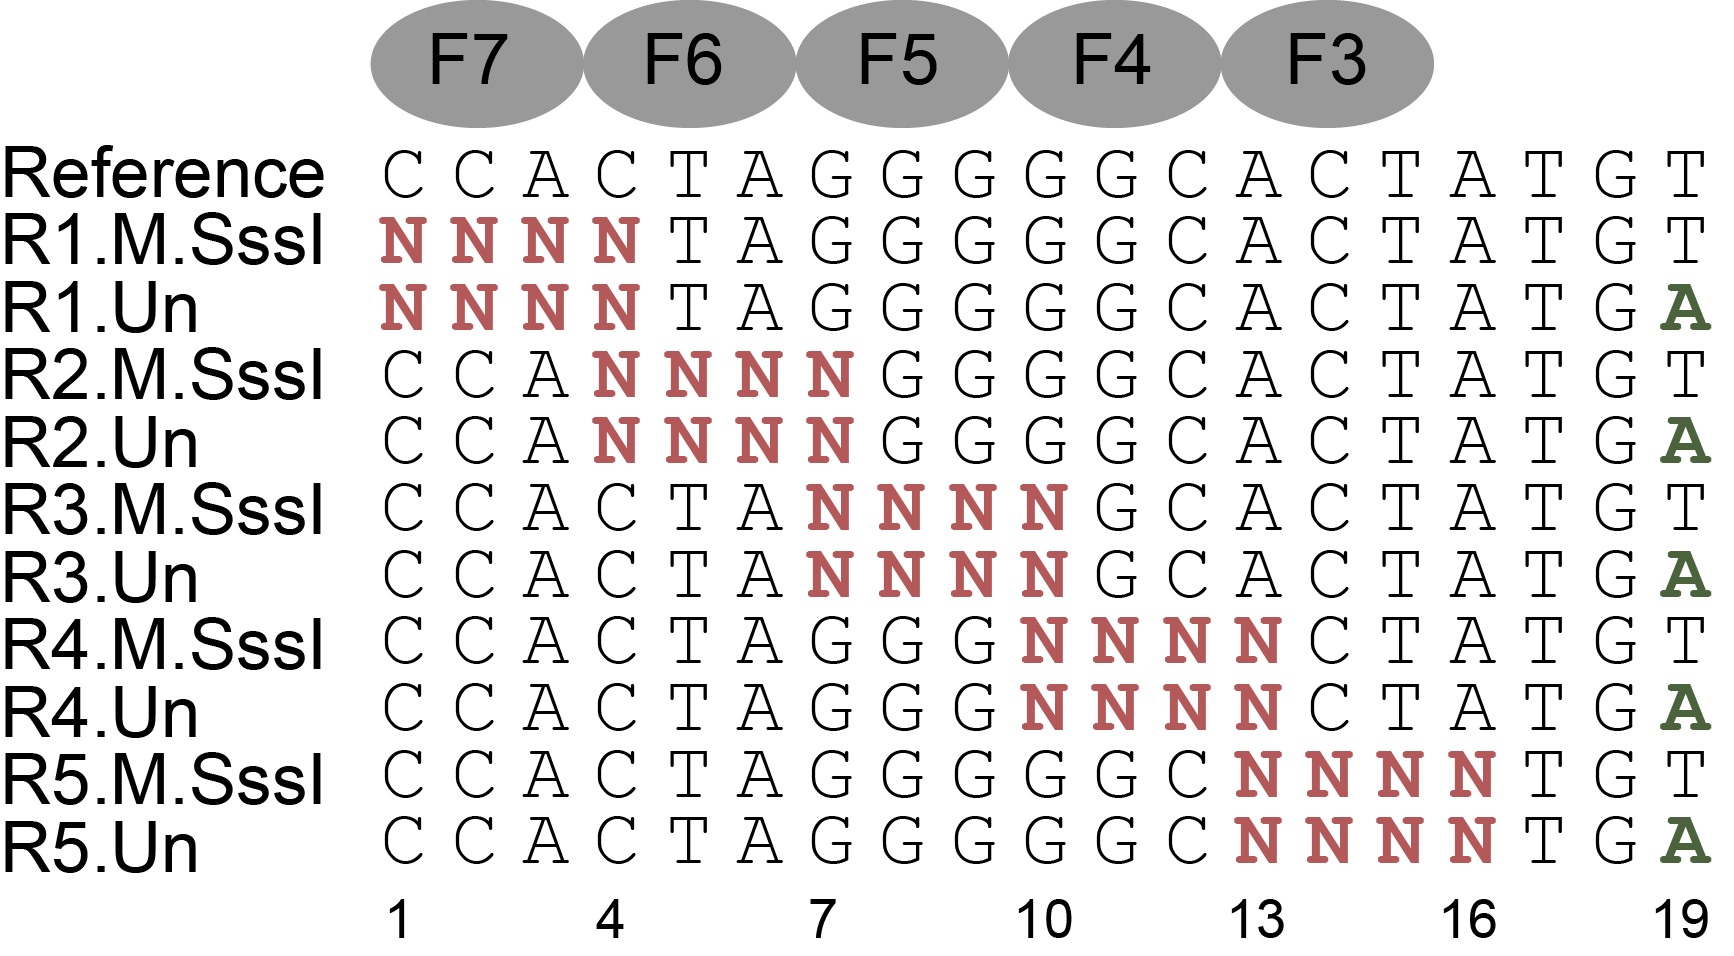
\includegraphics{./CTCF libraries design.png}

\hypertarget{importing-and-preprocessing-data}{%
\subsection{Importing and preprocessing
data}\label{importing-and-preprocessing-data}}

\begin{Shaded}
\begin{Highlighting}[]
\KeywordTok{load}\NormalTok{(}\StringTok{"../data/CTCF.rda"}\NormalTok{)}
\NormalTok{(CTCF \textless{}{-}}\StringTok{ }\NormalTok{CTCF }\OperatorTok{\%\textgreater{}\%}
\StringTok{  }\NormalTok{dplyr}\OperatorTok{::}\KeywordTok{mutate}\NormalTok{(}\StringTok{\textasciigrave{}}\DataTypeTok{Bound/Unbound}\StringTok{\textasciigrave{}}\NormalTok{ =}\StringTok{ }\NormalTok{Bound}\OperatorTok{/}\NormalTok{Unbound,}
                \DataTypeTok{Energy =} \OperatorTok{{-}}\KeywordTok{log}\NormalTok{(Bound}\OperatorTok{/}\NormalTok{Unbound)))}
\end{Highlighting}
\end{Shaded}

\begin{verbatim}
## # A tibble: 2,538 x 6
##    Sequence         Property Bound Unbound `Bound/Unbound` Energy
##    <chr>            <chr>    <dbl>   <dbl>           <dbl>  <dbl>
##  1 CCACTAGGGGGCGCTG me        3714     243            15.3  -2.73
##  2 CCACTAGGGGGCGCTG un        3184     232            13.7  -2.62
##  3 CCACTAGGGGGCGCTC un        2232     182            12.3  -2.51
##  4 CCACTAGGGGGCGCAC un        1494     127            11.8  -2.47
##  5 CCACTAGGGGGCGCTC me        1711     148            11.6  -2.45
##  6 CCACTAGGGGGCGCTA me       14185    1236            11.5  -2.44
##  7 CCACTAGGGGGCGCAG me        2408     210            11.5  -2.44
##  8 CCACTAGGGGGCGCAG un        2179     191            11.4  -2.43
##  9 CCACTAGGGGGCGCAA un        1577     139            11.3  -2.43
## 10 CCACTAGGGGGCGCCG me        2565     230            11.2  -2.41
## # ... with 2,528 more rows
\end{verbatim}

\hypertarget{building-regular-specificity-model-from-unmethylated-sites}{%
\subsection{Building regular specificity model from unmethylated
sites}\label{building-regular-specificity-model-from-unmethylated-sites}}

It is easy to build specificity model and derive motif based on energy
values from those unmethylated sites only.

\begin{Shaded}
\begin{Highlighting}[]
\NormalTok{CTCF.Model}\FloatTok{.3}\NormalTok{Lp1\textless{}{-}}\StringTok{ }\NormalTok{CTCF }\OperatorTok{\%\textgreater{}\%}
\StringTok{  }\NormalTok{dplyr}\OperatorTok{::}\KeywordTok{filter}\NormalTok{(Property }\OperatorTok{==}\StringTok{ "un"}\NormalTok{) }\OperatorTok{\%\textgreater{}\%}\StringTok{ }\CommentTok{\# Select those untreated sites}
\StringTok{  }\NormalTok{TFCookbook}\OperatorTok{::}\KeywordTok{buildEnergyModel}\NormalTok{(}\DataTypeTok{encoding =} \StringTok{"3L+1"}\NormalTok{)}

\NormalTok{CTCF.Model}\FloatTok{.3}\NormalTok{Lp1}\OperatorTok{\%\textgreater{}\%}
\StringTok{  }\NormalTok{TFCookbook}\OperatorTok{::}\KeywordTok{getEnergyMatrix}\NormalTok{() }\OperatorTok{\%\textgreater{}\%}
\StringTok{  }\NormalTok{TFCookbook}\OperatorTok{::}\KeywordTok{plotEnergyLogo}\NormalTok{() }\OperatorTok{+}
\StringTok{  }\KeywordTok{addFingers}\NormalTok{(}\DataTypeTok{index =} \DecValTok{7}\OperatorTok{:}\DecValTok{3}\NormalTok{, }\DataTypeTok{yMin =}  \FloatTok{{-}1.4}\NormalTok{, }\DataTypeTok{yMax =} \FloatTok{1.4}\NormalTok{) }\OperatorTok{+}
\StringTok{  }\KeywordTok{labs}\NormalTok{(}\DataTypeTok{title =} \StringTok{"Specificity profile of CTCF(F1{-}F9)}\CharTok{\textbackslash{}n}\StringTok{ based on energy values from unmethylated sites only"}\NormalTok{) }\OperatorTok{+}
\StringTok{  }\KeywordTok{theme}\NormalTok{(}\DataTypeTok{plot.title =} \KeywordTok{element\_text}\NormalTok{(}\DataTypeTok{hjust =} \FloatTok{0.5}\NormalTok{))}
\end{Highlighting}
\end{Shaded}

\includegraphics{CTCF-Analysis_files/figure-latex/unnamed-chunk-4-1.pdf}

\begin{Shaded}
\begin{Highlighting}[]
\CommentTok{\#ggsave("Regular motif.svg", plot = last\_plot(), height = 4.5, width = 9)}
\end{Highlighting}
\end{Shaded}

\hypertarget{building-methylation-sensitivity-model}{%
\subsection{Building Methylation Sensitivity
model}\label{building-methylation-sensitivity-model}}

\hypertarget{pairwise-comparison-of-unmethylated-sites-and-m.sssi-treated-sites}{%
\subsubsection{Pairwise comparison of unmethylated sites and M.SssI
treated
sites}\label{pairwise-comparison-of-unmethylated-sites-and-m.sssi-treated-sites}}

Since the designed libraries cover both M.SssI treated and untreated
sequences in one-to-one correspondence, it is possible to do pairwise
comparison for each site. Note that M.SssI treatment doesn't necessarily
mean methylation of cytosine, only those cytosines within CpG
dinucleotide can get methylated, therefore those CpG-non-containing
sequences can serve as negative control to gauge the intrinsic variances
of our Methyl-Spec-seq measurement.

\begin{Shaded}
\begin{Highlighting}[]
\NormalTok{CTCF.pairwise \textless{}{-}}\StringTok{ }\KeywordTok{inner\_join}\NormalTok{(}\KeywordTok{subset}\NormalTok{(CTCF, Property}\OperatorTok{==}\StringTok{"un"}\NormalTok{),}
                            \KeywordTok{subset}\NormalTok{(CTCF, Property}\OperatorTok{==}\StringTok{"me"}\NormalTok{), }\DataTypeTok{by =} \StringTok{"Sequence"}\NormalTok{) }\OperatorTok{\%\textgreater{}\%}
\StringTok{  }\NormalTok{dplyr}\OperatorTok{::}\KeywordTok{select}\NormalTok{(Sequence,}
                \DataTypeTok{Energy.un =} \StringTok{\textasciigrave{}}\DataTypeTok{Energy.x}\StringTok{\textasciigrave{}}\NormalTok{,}
                \DataTypeTok{Energy.me =} \StringTok{\textasciigrave{}}\DataTypeTok{Energy.y}\StringTok{\textasciigrave{}}\NormalTok{) }\OperatorTok{\%\textgreater{}\%}
\StringTok{  }\NormalTok{dplyr}\OperatorTok{::}\KeywordTok{mutate}\NormalTok{(}\DataTypeTok{CpG.containing =} \KeywordTok{as.integer}\NormalTok{(stringi}\OperatorTok{::}\KeywordTok{stri\_count\_fixed}\NormalTok{(Sequence, }\StringTok{"CG"}\NormalTok{)),}
                \DataTypeTok{Energy =}\NormalTok{ Energy.me }\OperatorTok{{-}}\StringTok{ }\NormalTok{Energy.un)}

\NormalTok{CTCF.pairwise }\OperatorTok{\%\textgreater{}\%}
\StringTok{  }\NormalTok{dplyr}\OperatorTok{::}\KeywordTok{arrange}\NormalTok{(}\KeywordTok{desc}\NormalTok{(Energy)) }\OperatorTok{\%\textgreater{}\%}
\StringTok{  }\NormalTok{dplyr}\OperatorTok{::}\KeywordTok{filter}\NormalTok{(Energy.un }\OperatorTok{\textless{}=}\StringTok{ }\FloatTok{1.5}\NormalTok{) }\OperatorTok{\%\textgreater{}\%}
\StringTok{  }\NormalTok{dplyr}\OperatorTok{::}\KeywordTok{rename}\NormalTok{(}\StringTok{\textasciigrave{}}\DataTypeTok{Number of CpG sites}\StringTok{\textasciigrave{}}\NormalTok{ =}\StringTok{ }\NormalTok{CpG.containing,}
                \StringTok{\textasciigrave{}}\DataTypeTok{Methylation effect (kT)}\StringTok{\textasciigrave{}}\NormalTok{ =}\StringTok{ }\NormalTok{Energy)}
\end{Highlighting}
\end{Shaded}

\begin{verbatim}
## # A tibble: 523 x 5
##    Sequence       Energy.un Energy.me `Number of CpG sit~ `Methylation effect (~
##    <chr>              <dbl>     <dbl>               <int>                  <dbl>
##  1 CCGGTAGGGGGCA~    -1.62     -0.488                   1                  1.13 
##  2 TCGCTAGGGGGCA~    -1.36     -1.01                    1                  0.343
##  3 CTCCTAGGGGGCA~     0.727     1.07                    0                  0.343
##  4 ACGGTAGGGGGCA~    -0.814    -0.489                   1                  0.325
##  5 CCGATAGGGGGCA~    -1.34     -1.07                    1                  0.273
##  6 CCACTAGGGCCCG~     1.23      1.49                    1                  0.258
##  7 CCACTAGGGGGCC~    -1.14     -0.891                   0                  0.247
##  8 CCACGAGGGGGCA~    -1.08     -0.842                   1                  0.242
##  9 TTACTAGGGGGCA~     1.30      1.53                    0                  0.234
## 10 CCACTAGGGGGCC~    -1.39     -1.16                    0                  0.227
## # ... with 513 more rows
\end{verbatim}

Clearly, for those high-affinity, or low-binding energy sequences,
C{CG}GTAGGGGGCACTA deviate significantly from the diagnoal lines by up
to \textasciitilde1kT, whereas almost all non-CpG containing sites fall
within the 0.25kT energy deviation bounds, so in our measurement mCpG at
position 2 significantly compromise the binding affinity of CTCF, which
is consistent with previous literature report. For those weak binding
sites, there are certain degree of divergence, very likely because of
the alternative recognition mode of CTCF including the nearby barcode
position, thus we consider that could be technical artifact.

\begin{Shaded}
\begin{Highlighting}[]
\NormalTok{CTCF.pairwise }\OperatorTok{\%\textgreater{}\%}
\StringTok{  }\NormalTok{dplyr}\OperatorTok{::}\KeywordTok{mutate}\NormalTok{(}\DataTypeTok{Label =} \KeywordTok{if\_else}\NormalTok{(}\KeywordTok{abs}\NormalTok{(Energy.un }\OperatorTok{{-}}\StringTok{ }\NormalTok{Energy.me)}\OperatorTok{\textgreater{}}\StringTok{ }\DecValTok{1}\NormalTok{, Sequence, }\StringTok{""}\NormalTok{), }
                \DataTypeTok{CpG.containing =} \KeywordTok{as.factor}\NormalTok{(CpG.containing)) }\OperatorTok{\%\textgreater{}\%}
\StringTok{  }\KeywordTok{ggplot}\NormalTok{(}\KeywordTok{aes}\NormalTok{(}\DataTypeTok{x =}\NormalTok{ Energy.un, }\DataTypeTok{y =}\NormalTok{ Energy.me, }\DataTypeTok{shape =}\NormalTok{ CpG.containing, }\DataTypeTok{color =}\NormalTok{ CpG.containing, }\DataTypeTok{label =}\NormalTok{ Label)) }\OperatorTok{+}
\StringTok{  }\KeywordTok{geom\_point}\NormalTok{() }\OperatorTok{+}
\StringTok{  }\KeywordTok{geom\_abline}\NormalTok{(}\DataTypeTok{intercept =} \FloatTok{{-}0.25}\NormalTok{, }\DataTypeTok{slope =} \DecValTok{1}\NormalTok{, }\DataTypeTok{linetype=}\StringTok{"dashed"}\NormalTok{) }\OperatorTok{+}
\StringTok{  }\KeywordTok{geom\_abline}\NormalTok{(}\DataTypeTok{intercept =} \FloatTok{0.25}\NormalTok{, }\DataTypeTok{slope =} \DecValTok{1}\NormalTok{, }\DataTypeTok{linetype=}\StringTok{"dashed"}\NormalTok{) }\OperatorTok{+}
\StringTok{  }\KeywordTok{geom\_text\_repel}\NormalTok{(}\DataTypeTok{show.legend =} \OtherTok{FALSE}\NormalTok{, }\DataTypeTok{force =} \DecValTok{10}\NormalTok{) }\OperatorTok{+}
\StringTok{  }\KeywordTok{ggtitle}\NormalTok{(}\StringTok{"Binding energy comparison between M.SssI treated and untreated sites"}\NormalTok{) }\OperatorTok{+}
\StringTok{  }\KeywordTok{scale\_x\_continuous}\NormalTok{(}\DataTypeTok{breaks =} \KeywordTok{seq}\NormalTok{(}\OperatorTok{{-}}\DecValTok{2}\NormalTok{, }\DecValTok{4}\NormalTok{, }\DecValTok{1}\NormalTok{)) }\OperatorTok{+}\StringTok{ }\KeywordTok{scale\_y\_continuous}\NormalTok{(}\DataTypeTok{breaks =} \KeywordTok{seq}\NormalTok{(}\OperatorTok{{-}}\DecValTok{2}\NormalTok{, }\DecValTok{4}\NormalTok{, }\DecValTok{1}\NormalTok{)) }\OperatorTok{+}
\StringTok{  }\KeywordTok{xlab}\NormalTok{(}\StringTok{"Binding energy for untreated sites (kT)"}\NormalTok{) }\OperatorTok{+}
\StringTok{  }\KeywordTok{ylab}\NormalTok{(}\StringTok{"Binding energy for M.SssI treated sites (kT)"}\NormalTok{) }\OperatorTok{+}
\StringTok{  }\KeywordTok{labs}\NormalTok{(}\DataTypeTok{shape =} \StringTok{"Number of CpGs within sequence"}\NormalTok{, }\DataTypeTok{color =} \StringTok{"Number of CpGs within sequence"}\NormalTok{) }\OperatorTok{+}
\StringTok{  }\KeywordTok{theme}\NormalTok{(}\DataTypeTok{legend.position =} \StringTok{"bottom"}\NormalTok{, }\DataTypeTok{plot.title =} \KeywordTok{element\_text}\NormalTok{(}\DataTypeTok{hjust =} \FloatTok{0.5}\NormalTok{))}
\end{Highlighting}
\end{Shaded}

\includegraphics{CTCF-Analysis_files/figure-latex/unnamed-chunk-6-1.pdf}

\begin{Shaded}
\begin{Highlighting}[]
\CommentTok{\#ggsave("Pairwise comparison.svg", plot = last\_plot(), height = 5.7, width = 8)}
\end{Highlighting}
\end{Shaded}

\hypertarget{building-methylation-sensitivity-model-by-regression-of-4l1-parameters-all-together}{%
\subsubsection{Building Methylation sensitivity model by regression of
4L+1 parameters all
together}\label{building-methylation-sensitivity-model-by-regression-of-4l1-parameters-all-together}}

As discussed in the main text, if we use encoding scheme (3+1)L+1 and do
regression analysis with all 4L+1 parameters altegether, we can get some
methylation profiles shown below, which is very different from what we
expect based on visual inspection, e.g., position 2 didn't show any
negative methylation sensitivity at all and other positions show
considerable ammount of methyl effect.

\begin{Shaded}
\begin{Highlighting}[]
\NormalTok{CTCF.Model}\FloatTok{.4}\NormalTok{Lp1 \textless{}{-}}\StringTok{ }\NormalTok{CTCF }\OperatorTok{\%\textgreater{}\%}
\StringTok{  }\NormalTok{dplyr}\OperatorTok{::}\KeywordTok{mutate}\NormalTok{(}\DataTypeTok{Sequence =} \KeywordTok{if\_else}\NormalTok{(Property}\OperatorTok{==}\StringTok{"un"}\NormalTok{,}
\NormalTok{                                   Sequence,}
\NormalTok{                                   stringi}\OperatorTok{::}\KeywordTok{stri\_replace\_all\_fixed}\NormalTok{(Sequence, }\StringTok{"CG"}\NormalTok{, }\StringTok{"MW"}\NormalTok{))) }\OperatorTok{\%\textgreater{}\%}
\StringTok{  }\NormalTok{dplyr}\OperatorTok{::}\KeywordTok{filter}\NormalTok{(Energy }\OperatorTok{\textless{}=}\StringTok{ }\FloatTok{1.7}\NormalTok{) }\OperatorTok{\%\textgreater{}\%}
\StringTok{  }\NormalTok{TFCookbook}\OperatorTok{::}\KeywordTok{buildEnergyModel}\NormalTok{(}\DataTypeTok{encoding =} \StringTok{"4L+1"}\NormalTok{)}
  
\NormalTok{CTCF.Model}\FloatTok{.4}\NormalTok{Lp1 }\OperatorTok{\%\textgreater{}\%}
\StringTok{  }\NormalTok{TFCookbook}\OperatorTok{::}\KeywordTok{getEnergyMatrix}\NormalTok{() }\OperatorTok{\%\textgreater{}\%}
\StringTok{  }\NormalTok{TFCookbook}\OperatorTok{::}\KeywordTok{addMethylMatrix}\NormalTok{(CTCF.Model}\FloatTok{.4}\NormalTok{Lp1, }\DataTypeTok{encoding =} \StringTok{"(3+1)L+1"}\NormalTok{) }\OperatorTok{\%\textgreater{}\%}
\StringTok{  }\NormalTok{TFCookbook}\OperatorTok{::}\KeywordTok{plotEnergyLogo}\NormalTok{() }\OperatorTok{+}
\StringTok{  }\KeywordTok{addFingers}\NormalTok{(}\DataTypeTok{index =} \DecValTok{7}\OperatorTok{:}\DecValTok{3}\NormalTok{, }\FloatTok{{-}1.6}\NormalTok{, }\FloatTok{2.45}\NormalTok{) }\OperatorTok{+}
\StringTok{  }\KeywordTok{scale\_y\_continuous}\NormalTok{(}\DataTypeTok{breaks =} \KeywordTok{seq}\NormalTok{(}\OperatorTok{{-}}\FloatTok{1.5}\NormalTok{, }\DecValTok{2}\NormalTok{, }\FloatTok{0.5}\NormalTok{)) }\OperatorTok{+}
\StringTok{  }\KeywordTok{labs}\NormalTok{(}\DataTypeTok{title =} \StringTok{"Specificity profile of CTCF(F1{-}F9) }
\StringTok{       by regression with specificity and methylation parameters together"}\NormalTok{) }\OperatorTok{+}
\StringTok{  }\KeywordTok{theme}\NormalTok{(}\DataTypeTok{plot.title =} \KeywordTok{element\_text}\NormalTok{(}\DataTypeTok{hjust =} \FloatTok{0.5}\NormalTok{))}
\end{Highlighting}
\end{Shaded}

\includegraphics{CTCF-Analysis_files/figure-latex/unnamed-chunk-7-1.pdf}

\begin{Shaded}
\begin{Highlighting}[]
\CommentTok{\#ggsave("4L+1 motif.svg", plot = last\_plot(), height = 4.5, width = 9)}
\end{Highlighting}
\end{Shaded}

\hypertarget{building-methylation-sensitivity-model-by-separate-evaluation-of-methylation-effect-on-each-binding-site}{%
\subsubsection{Building Methylation sensitivity model by separate
evaluation of methylation effect on each binding
site}\label{building-methylation-sensitivity-model-by-separate-evaluation-of-methylation-effect-on-each-binding-site}}

Alternatively, if we perform regression over methylation-related
parameters (1MW to 16MW) alone using pairwise comparison data, it is
easy to derive a methylation sensitivity model that matches our visual
inspection well. Note that our measurement resolution is around 0.25kT,
so we can choose 0.25kT as cut-off to analyze those significant
methylation effect alone.

\begin{Shaded}
\begin{Highlighting}[]
\NormalTok{(CTCF.MethylModel \textless{}{-}}\StringTok{ }\NormalTok{CTCF.pairwise }\OperatorTok{\%\textgreater{}\%}
\StringTok{  }\KeywordTok{filter}\NormalTok{(Energy.un }\OperatorTok{\textless{}=}\StringTok{ }\FloatTok{1.5}\NormalTok{, Energy }\OperatorTok{\textgreater{}}\StringTok{ }\FloatTok{0.25}\NormalTok{) }\OperatorTok{\%\textgreater{}\%}\StringTok{ }\CommentTok{\#\# Filtering out low affinity binding sites and select only significant observation}
\StringTok{  }\KeywordTok{mutate}\NormalTok{(}\DataTypeTok{Sequence =}\NormalTok{ stringi}\OperatorTok{::}\KeywordTok{stri\_replace\_all\_fixed}\NormalTok{(Sequence, }\StringTok{"CG"}\NormalTok{, }\StringTok{"MW"}\NormalTok{)) }\OperatorTok{\%\textgreater{}\%}
\StringTok{  }\KeywordTok{arrange}\NormalTok{(}\KeywordTok{desc}\NormalTok{(Energy)) }\OperatorTok{\%\textgreater{}\%}
\StringTok{  }\NormalTok{TFCookbook}\OperatorTok{::}\KeywordTok{buildMethylationModel}\NormalTok{(}\DataTypeTok{encoding =} \StringTok{"(3+1)L+1"}\NormalTok{, }\DataTypeTok{withIntercept =} \OtherTok{FALSE}\NormalTok{))}
\end{Highlighting}
\end{Shaded}

\begin{verbatim}
## 
## Call:
## lm(formula = Energy ~ . - Energy + 0, data = input)
## 
## Coefficients:
##  `1MW`   `2MW`   `3MW`   `4MW`   `5MW`   `6MW`   `7MW`   `8MW`   `9MW`  `10MW`  
##     NA  0.5174      NA      NA      NA      NA      NA      NA      NA      NA  
## `11MW`  `12MW`  `13MW`  `14MW`  `15MW`  `16MW`  
##     NA  0.2582      NA      NA      NA      NA
\end{verbatim}

By combining specificity and methylation sensitivity info together, we
can produce some motif logo that catches most of information to our
expectation. Since we have no information about the strand-specific
methylation effect in current experimetal setup, we just plot it as
50/50 by default. It has been shown in other literature that the
methylation effect at position (2,3) primarily comes from the upper
strand.

\begin{Shaded}
\begin{Highlighting}[]
\NormalTok{CTCF.Model}\FloatTok{.3}\NormalTok{Lp1}\OperatorTok{\%\textgreater{}\%}
\StringTok{  }\NormalTok{TFCookbook}\OperatorTok{::}\KeywordTok{getEnergyMatrix}\NormalTok{() }\OperatorTok{\%\textgreater{}\%}\StringTok{  }\CommentTok{\#\# Getting energy matrix for regular specificity model}
\StringTok{  }\NormalTok{TFCookbook}\OperatorTok{::}\KeywordTok{addMethylMatrix}\NormalTok{(CTCF.MethylModel, }\DataTypeTok{encoding =} \StringTok{"(3+1)L+1"}\NormalTok{) }\OperatorTok{\%\textgreater{}\%}\StringTok{ }\CommentTok{\#\# Adding methylation parameters to the matrix}
\StringTok{  }\NormalTok{TFCookbook}\OperatorTok{::}\KeywordTok{plotEnergyLogo}\NormalTok{() }\OperatorTok{+}
\StringTok{  }\KeywordTok{addFingers}\NormalTok{(}\DataTypeTok{index =} \DecValTok{7}\OperatorTok{:}\DecValTok{3}\NormalTok{, }\FloatTok{{-}1.5}\NormalTok{, }\FloatTok{1.4}\NormalTok{) }\OperatorTok{+}
\StringTok{  }\KeywordTok{scale\_y\_continuous}\NormalTok{(}\DataTypeTok{breaks =} \KeywordTok{seq}\NormalTok{(}\OperatorTok{{-}}\FloatTok{1.5}\NormalTok{, }\FloatTok{1.5}\NormalTok{, }\FloatTok{0.5}\NormalTok{)) }\OperatorTok{+}
\StringTok{  }\KeywordTok{labs}\NormalTok{(}\DataTypeTok{title =} \StringTok{"Specificity profile of CTCF(F1{-}F9)}
\StringTok{       by separate regression with specificity and methylation parameters respectively"}\NormalTok{) }\OperatorTok{+}
\StringTok{  }\KeywordTok{theme}\NormalTok{(}\DataTypeTok{plot.title =} \KeywordTok{element\_text}\NormalTok{(}\DataTypeTok{hjust =} \FloatTok{0.5}\NormalTok{))}
\end{Highlighting}
\end{Shaded}

\includegraphics{CTCF-Analysis_files/figure-latex/unnamed-chunk-9-1.pdf}

\begin{Shaded}
\begin{Highlighting}[]
\CommentTok{\#ggsave("Separate regressions motif.svg", plot = last\_plot(), height = 4.5, width = 9)}
\end{Highlighting}
\end{Shaded}

\hypertarget{why-separate-regression-over-specificity-and-methylation-data-performs-better-than-all-in-one-regression}{%
\subsubsection{Why separate regression over specificity and methylation
data performs better than all-in-one
regression?}\label{why-separate-regression-over-specificity-and-methylation-data-performs-better-than-all-in-one-regression}}

To illustrate the intrinsic limitation of all-in-one regresson of all
parameters, we can compare all those predicted binding energy for
unmethylated and methylated sites at each position based on 4L+1 model
with the observed values as following figure. Clearly, for those
sequences with CpG at position 1 and 11, each pair exhibited almost no
methylation effect, but we still get non-zero methylation parameters
(1MW and 11MW), most likely because non-zero methyl- parameters
decreases the overall deviation between observed and predicted values
and ``push'' most pairs closer to the diagnoal lines. On the other hand,
for sequences with CpG at position 2, only one sequence
(CCGGTAGGGGGCACTA) showed significant methylation effect, which gets
``buried'' in other insignificant ones, and thus we couldn't get some
positive 2MW parameter with 4L+1 regression method.

\begin{Shaded}
\begin{Highlighting}[]
\NormalTok{CTCF}\FloatTok{.4}\NormalTok{Lp1 \textless{}{-}}\StringTok{ }\NormalTok{CTCF }\OperatorTok{\%\textgreater{}\%}
\StringTok{  }\NormalTok{dplyr}\OperatorTok{::}\KeywordTok{mutate}\NormalTok{(}\DataTypeTok{position.CpG =}\NormalTok{ stringi}\OperatorTok{::}\KeywordTok{stri\_locate\_first\_fixed}\NormalTok{(Sequence, }\StringTok{"CG"}\NormalTok{)[,}\StringTok{"start"}\NormalTok{]) }\OperatorTok{\%\textgreater{}\%}
\StringTok{  }\NormalTok{dplyr}\OperatorTok{::}\KeywordTok{filter}\NormalTok{(Energy }\OperatorTok{\textless{}=}\StringTok{ }\FloatTok{1.7}\NormalTok{) }\OperatorTok{\%\textgreater{}\%}
\StringTok{  }\NormalTok{dplyr}\OperatorTok{::}\KeywordTok{mutate}\NormalTok{(}\DataTypeTok{Predicted.Energy =}\NormalTok{ CTCF.Model}\FloatTok{.4}\NormalTok{Lp1}\OperatorTok{$}\NormalTok{fitted.values) }\CommentTok{\#\#Adding predicted values by 4L+1 regression method}

\NormalTok{CTCF}\FloatTok{.4}\NormalTok{Lp1.paired \textless{}{-}}\StringTok{ }
\StringTok{    }\NormalTok{dplyr}\OperatorTok{::}\KeywordTok{inner\_join}\NormalTok{(}\KeywordTok{subset}\NormalTok{(CTCF}\FloatTok{.4}\NormalTok{Lp1, Property }\OperatorTok{==}\StringTok{ "un"}\NormalTok{),}
                      \KeywordTok{subset}\NormalTok{(CTCF}\FloatTok{.4}\NormalTok{Lp1, Property }\OperatorTok{==}\StringTok{ "me"}\NormalTok{),}
                      \DataTypeTok{by =} \StringTok{"Sequence"}\NormalTok{) }\OperatorTok{\%\textgreater{}\%}
\StringTok{    }\NormalTok{dplyr}\OperatorTok{::}\KeywordTok{select}\NormalTok{(Sequence,}
                  \DataTypeTok{position.CpG =}\NormalTok{ position.CpG.x,}
                  \DataTypeTok{Energy.un =}\NormalTok{ Energy.x,}
                  \DataTypeTok{Predicted.Energy.un =}\NormalTok{ Predicted.Energy.x,}
                  \DataTypeTok{Energy.me =}\NormalTok{ Energy.y,}
                  \DataTypeTok{Predicted.Energy.me =}\NormalTok{ Predicted.Energy.y)}

\NormalTok{CTCF}\FloatTok{.4}\NormalTok{Lp1.paired }\OperatorTok{\%\textgreater{}\%}
\StringTok{    }\NormalTok{dplyr}\OperatorTok{::}\KeywordTok{filter}\NormalTok{(position.CpG }\OperatorTok{\%in\%}\StringTok{ }\KeywordTok{c}\NormalTok{(}\DecValTok{1}\NormalTok{, }\DecValTok{2}\NormalTok{, }\DecValTok{11}\NormalTok{)) }\OperatorTok{\%\textgreater{}\%}
\StringTok{    }\KeywordTok{ggplot}\NormalTok{() }\OperatorTok{+}
\StringTok{    }\KeywordTok{geom\_abline}\NormalTok{(}\DataTypeTok{intercept =} \DecValTok{0}\NormalTok{, }\DataTypeTok{slope =} \DecValTok{1}\NormalTok{, }\DataTypeTok{linetype =} \StringTok{"dashed"}\NormalTok{) }\OperatorTok{+}
\StringTok{    }\KeywordTok{geom\_point}\NormalTok{(}\KeywordTok{aes}\NormalTok{(}\DataTypeTok{x =}\NormalTok{ Predicted.Energy.un, }\DataTypeTok{y =}\NormalTok{ Energy.un), }\DataTypeTok{color =} \StringTok{"blue"}\NormalTok{, }\DataTypeTok{shape =} \DecValTok{0}\NormalTok{) }\OperatorTok{+}
\StringTok{    }\KeywordTok{geom\_point}\NormalTok{(}\KeywordTok{aes}\NormalTok{(}\DataTypeTok{x =}\NormalTok{ Predicted.Energy.me, }\DataTypeTok{y =}\NormalTok{ Energy.me), }\DataTypeTok{color =} \StringTok{"red"}\NormalTok{, }\DataTypeTok{shape =} \DecValTok{19}\NormalTok{) }\OperatorTok{+}
\StringTok{    }\KeywordTok{geom\_segment}\NormalTok{(}\KeywordTok{aes}\NormalTok{(}\DataTypeTok{x =}\NormalTok{ Predicted.Energy.un, }\DataTypeTok{y =}\NormalTok{ Energy.un,}
                     \DataTypeTok{xend =}\NormalTok{ Predicted.Energy.me, }\DataTypeTok{yend =}\NormalTok{ Energy.me),}
                 \DataTypeTok{lineend =} \StringTok{\textquotesingle{}round\textquotesingle{}}\NormalTok{, }\DataTypeTok{linejoin =} \StringTok{\textquotesingle{}bevel\textquotesingle{}}\NormalTok{, }\DataTypeTok{size =} \DecValTok{1}\NormalTok{, }\DataTypeTok{color =} \StringTok{"orange"}\NormalTok{,}
                 \DataTypeTok{arrow =} \KeywordTok{arrow}\NormalTok{(}\DataTypeTok{length =} \KeywordTok{unit}\NormalTok{(}\FloatTok{0.03}\NormalTok{, }\StringTok{"npc"}\NormalTok{))) }\OperatorTok{+}
\StringTok{    }\KeywordTok{geom\_text\_repel}\NormalTok{(}\DataTypeTok{data =} \ControlFlowTok{function}\NormalTok{(x) }\KeywordTok{filter}\NormalTok{(x, ((position.CpG }\OperatorTok{!=}\StringTok{ }\DecValTok{2}\NormalTok{) }\OperatorTok{|}\StringTok{ }\NormalTok{(Sequence }\OperatorTok{==}\StringTok{ "CCGGTAGGGGGCACTA"}\NormalTok{))),}
                    \KeywordTok{aes}\NormalTok{(}\DataTypeTok{x =}\NormalTok{ Predicted.Energy.un, }\DataTypeTok{y =}\NormalTok{ Energy.un, }\DataTypeTok{label =}\NormalTok{ Sequence), }\DataTypeTok{force =} \DecValTok{1}\NormalTok{) }\OperatorTok{+}
\StringTok{    }\KeywordTok{ggtitle}\NormalTok{(}\StringTok{"Comparison of experimental data with predicted values by 4L+1 model"}\NormalTok{) }\OperatorTok{+}
\StringTok{    }\KeywordTok{xlab}\NormalTok{(}\StringTok{"Predicted binding energy by regression of (4L+1) parameters together (kT)"}\NormalTok{) }\OperatorTok{+}
\StringTok{    }\KeywordTok{ylab}\NormalTok{(}\StringTok{"Observed binding energy (kT)"}\NormalTok{) }\OperatorTok{+}
\StringTok{    }\KeywordTok{facet\_wrap}\NormalTok{(}\OperatorTok{\textasciitilde{}}\NormalTok{position.CpG, }
               \DataTypeTok{scales =} \StringTok{"free\_y"}\NormalTok{,}
               \DataTypeTok{strip.position =} \StringTok{"right"}\NormalTok{,}
               \DataTypeTok{nrow =} \DecValTok{3}\NormalTok{)}
\end{Highlighting}
\end{Shaded}

\includegraphics{CTCF-Analysis_files/figure-latex/unnamed-chunk-10-1.pdf}

\begin{Shaded}
\begin{Highlighting}[]
\CommentTok{\#ggsave("Model 4Lp1 comparison.svg", plot = last\_plot(), height = 9, width = 7)}
\end{Highlighting}
\end{Shaded}

\hypertarget{l1-modeling-with-artificial-data-exhibits-the-intrinsic-limitation-of-all-in-one-regression-strategy}{%
\subsubsection{4L+1 modeling with artificial data exhibits the intrinsic
limitation of all-in-one regression
strategy}\label{l1-modeling-with-artificial-data-exhibits-the-intrinsic-limitation-of-all-in-one-regression-strategy}}

Besides comparison of experimental data with predicted values by 4L+1
model, we can create an artificial ``pseudo'' dataset in which each
methylated site has exactly the same value as the unmethylated one, and
construct 4L+1 model to illustrate the intrinsic limitation of this
all-in-one regression strategy.

\begin{Shaded}
\begin{Highlighting}[]
\NormalTok{CTCF.pseudoMe \textless{}{-}}\StringTok{ }\KeywordTok{subset}\NormalTok{(CTCF, Property }\OperatorTok{==}\StringTok{ "un"}\NormalTok{) }\OperatorTok{\%\textgreater{}\%}
\StringTok{  }\NormalTok{dplyr}\OperatorTok{::}\KeywordTok{mutate}\NormalTok{(}\DataTypeTok{Sequence =}\NormalTok{ stringi}\OperatorTok{::}\KeywordTok{stri\_replace\_all\_fixed}\NormalTok{(Sequence, }\StringTok{"CG"}\NormalTok{, }\StringTok{"MW"}\NormalTok{),}
                \DataTypeTok{Property =} \StringTok{"me"}\NormalTok{) }\OperatorTok{\%\textgreater{}\%}
\StringTok{  }\NormalTok{dplyr}\OperatorTok{::}\KeywordTok{filter}\NormalTok{(stringr}\OperatorTok{::}\KeywordTok{str\_detect}\NormalTok{(Sequence, }\StringTok{"MW"}\NormalTok{))}

\NormalTok{CTCF.pseudoModel}\FloatTok{.4}\NormalTok{Lp1 \textless{}{-}}\StringTok{  }\KeywordTok{rbind}\NormalTok{(}\KeywordTok{subset}\NormalTok{(CTCF, Property }\OperatorTok{==}\StringTok{ "un"}\NormalTok{), CTCF.pseudoMe) }\OperatorTok{\%\textgreater{}\%}
\StringTok{  }\NormalTok{TFCookbook}\OperatorTok{::}\KeywordTok{buildEnergyModel}\NormalTok{(}\DataTypeTok{encoding =} \StringTok{"4L+1"}\NormalTok{)}

\NormalTok{CTCF.pseudoModel}\FloatTok{.4}\NormalTok{Lp1 }\OperatorTok{\%\textgreater{}\%}
\StringTok{  }\NormalTok{TFCookbook}\OperatorTok{::}\KeywordTok{getEnergyMatrix}\NormalTok{() }\OperatorTok{\%\textgreater{}\%}
\StringTok{  }\NormalTok{TFCookbook}\OperatorTok{::}\KeywordTok{addMethylMatrix}\NormalTok{(}\DataTypeTok{MethylModel =}\NormalTok{ CTCF.pseudoModel}\FloatTok{.4}\NormalTok{Lp1, }\DataTypeTok{encoding =} \StringTok{"(3+1)L+1"}\NormalTok{) }\OperatorTok{\%\textgreater{}\%}
\StringTok{  }\NormalTok{TFCookbook}\OperatorTok{::}\KeywordTok{plotEnergyLogo}\NormalTok{() }\OperatorTok{+}
\StringTok{  }\KeywordTok{addFingers}\NormalTok{(}\DataTypeTok{index =} \DecValTok{7}\OperatorTok{:}\DecValTok{3}\NormalTok{, }\FloatTok{{-}1.6}\NormalTok{, }\FloatTok{1.6}\NormalTok{) }\OperatorTok{+}
\StringTok{  }\KeywordTok{scale\_y\_continuous}\NormalTok{(}\DataTypeTok{breaks =} \KeywordTok{seq}\NormalTok{(}\OperatorTok{{-}}\FloatTok{1.5}\NormalTok{, }\FloatTok{1.5}\NormalTok{, }\FloatTok{0.5}\NormalTok{)) }\OperatorTok{+}
\StringTok{  }\KeywordTok{labs}\NormalTok{(}\DataTypeTok{title =} \StringTok{"Pseudo Specificity profile of CTCF(F1{-}F9) }
\StringTok{       by regression with specificity and methylation parameters together"}\NormalTok{) }\OperatorTok{+}
\StringTok{  }\KeywordTok{theme}\NormalTok{(}\DataTypeTok{plot.title =} \KeywordTok{element\_text}\NormalTok{(}\DataTypeTok{hjust =} \FloatTok{0.5}\NormalTok{))}
\end{Highlighting}
\end{Shaded}

\includegraphics{CTCF-Analysis_files/figure-latex/unnamed-chunk-11-1.pdf}

Clearly, under this ``absolute no methylation effect'' scenario, we
still derive some non-zero methylation parameters from 4L+1 model, which
shows us it is more realistic to build separate methylation effect model
based on pairwise comparison between each individual site.

\begin{Shaded}
\begin{Highlighting}[]
\NormalTok{CTCF.pseudo.paired \textless{}{-}}\StringTok{ }\KeywordTok{subset}\NormalTok{(CTCF, Property }\OperatorTok{==}\StringTok{ "un"}\NormalTok{) }\OperatorTok{\%\textgreater{}\%}
\StringTok{  }\NormalTok{dplyr}\OperatorTok{::}\KeywordTok{mutate}\NormalTok{(}\DataTypeTok{Sequence.MW =}\NormalTok{ stringi}\OperatorTok{::}\KeywordTok{stri\_replace\_all\_fixed}\NormalTok{(Sequence, }\StringTok{"CG"}\NormalTok{, }\StringTok{"MW"}\NormalTok{),}
                \DataTypeTok{position.CpG =}\NormalTok{ stringi}\OperatorTok{::}\KeywordTok{stri\_locate\_first\_fixed}\NormalTok{(Sequence, }\StringTok{"CG"}\NormalTok{)[,}\StringTok{"start"}\NormalTok{],}
                \DataTypeTok{Predicted.Energy.un =}\NormalTok{ TFCookbook}\OperatorTok{::}\KeywordTok{predictEnergyMW}\NormalTok{(Sequence, CTCF.pseudoModel}\FloatTok{.4}\NormalTok{Lp1),}
                \DataTypeTok{Predicted.Energy.me =}\NormalTok{ TFCookbook}\OperatorTok{::}\KeywordTok{predictEnergyMW}\NormalTok{(Sequence.MW, CTCF.pseudoModel}\FloatTok{.4}\NormalTok{Lp1)) }\OperatorTok{\%\textgreater{}\%}
\StringTok{  }\NormalTok{dplyr}\OperatorTok{::}\KeywordTok{select}\NormalTok{(Sequence, Sequence.MW, position.CpG, Energy, Predicted.Energy.un, Predicted.Energy.me)}
\end{Highlighting}
\end{Shaded}

\begin{verbatim}
## Warning: Expected 64 pieces. Additional pieces discarded in 1266 rows [1, 2, 3,
## 4, 5, 6, 7, 8, 9, 10, 11, 12, 13, 14, 15, 16, 17, 18, 19, 20, ...].
\end{verbatim}

\begin{verbatim}
## Warning in predict.lm(model, newdata = ., type = "response"): prediction from a
## rank-deficient fit may be misleading
\end{verbatim}

\begin{verbatim}
## Warning: Expected 64 pieces. Additional pieces discarded in 1266 rows [1, 2, 3,
## 4, 5, 6, 7, 8, 9, 10, 11, 12, 13, 14, 15, 16, 17, 18, 19, 20, ...].
\end{verbatim}

\begin{verbatim}
## Warning in predict.lm(model, newdata = ., type = "response"): prediction from a
## rank-deficient fit may be misleading
\end{verbatim}

\begin{Shaded}
\begin{Highlighting}[]
\NormalTok{CTCF.pseudo.paired }\OperatorTok{\%\textgreater{}\%}
\StringTok{    }\NormalTok{dplyr}\OperatorTok{::}\KeywordTok{filter}\NormalTok{(position.CpG }\OperatorTok{\%in\%}\StringTok{ }\KeywordTok{c}\NormalTok{(}\DecValTok{1}\NormalTok{, }\DecValTok{2}\NormalTok{, }\DecValTok{11}\NormalTok{)) }\OperatorTok{\%\textgreater{}\%}
\StringTok{    }\KeywordTok{ggplot}\NormalTok{() }\OperatorTok{+}
\StringTok{    }\KeywordTok{geom\_abline}\NormalTok{(}\DataTypeTok{intercept =} \DecValTok{0}\NormalTok{, }\DataTypeTok{slope =} \DecValTok{1}\NormalTok{, }\DataTypeTok{linetype =} \StringTok{"dashed"}\NormalTok{) }\OperatorTok{+}
\StringTok{    }\KeywordTok{geom\_point}\NormalTok{(}\KeywordTok{aes}\NormalTok{(}\DataTypeTok{x =}\NormalTok{ Predicted.Energy.un, }\DataTypeTok{y =}\NormalTok{ Energy), }\DataTypeTok{color =} \StringTok{"blue"}\NormalTok{, }\DataTypeTok{shape =} \DecValTok{0}\NormalTok{) }\OperatorTok{+}
\StringTok{    }\KeywordTok{geom\_point}\NormalTok{(}\KeywordTok{aes}\NormalTok{(}\DataTypeTok{x =}\NormalTok{ Predicted.Energy.me, }\DataTypeTok{y =}\NormalTok{ Energy), }\DataTypeTok{color =} \StringTok{"red"}\NormalTok{, }\DataTypeTok{shape =} \DecValTok{19}\NormalTok{) }\OperatorTok{+}
\StringTok{    }\KeywordTok{geom\_segment}\NormalTok{(}\KeywordTok{aes}\NormalTok{(}\DataTypeTok{x =}\NormalTok{ Predicted.Energy.un, }\DataTypeTok{y =}\NormalTok{ Energy,}
                     \DataTypeTok{xend =}\NormalTok{ Predicted.Energy.me, }\DataTypeTok{yend =}\NormalTok{ Energy),}
                 \DataTypeTok{lineend =} \StringTok{\textquotesingle{}round\textquotesingle{}}\NormalTok{, }\DataTypeTok{linejoin =} \StringTok{\textquotesingle{}bevel\textquotesingle{}}\NormalTok{, }\DataTypeTok{size =} \DecValTok{1}\NormalTok{, }\DataTypeTok{color =} \StringTok{"orange"}\NormalTok{,}
                 \DataTypeTok{arrow =} \KeywordTok{arrow}\NormalTok{(}\DataTypeTok{length =} \KeywordTok{unit}\NormalTok{(}\FloatTok{0.03}\NormalTok{, }\StringTok{"npc"}\NormalTok{))) }\OperatorTok{+}
\StringTok{   }\CommentTok{\#\# geom\_text\_repel(aes(x = Predicted.Energy.un, y = Energy, label = Sequence)) +}
\StringTok{    }\KeywordTok{ggtitle}\NormalTok{(}\StringTok{"Comparison of artifical data with predicted values by 4L+1 model"}\NormalTok{) }\OperatorTok{+}
\StringTok{    }\KeywordTok{xlab}\NormalTok{(}\StringTok{"Predicted binding energy by 4L+1 model (kT)"}\NormalTok{) }\OperatorTok{+}
\StringTok{    }\KeywordTok{ylab}\NormalTok{(}\StringTok{"Observed binding energy (kT)"}\NormalTok{) }\OperatorTok{+}
\StringTok{    }\KeywordTok{facet\_wrap}\NormalTok{(}\OperatorTok{\textasciitilde{}}\NormalTok{position.CpG, }
               \DataTypeTok{scales =} \StringTok{"free\_y"}\NormalTok{,}
               \DataTypeTok{strip.position =} \StringTok{"right"}\NormalTok{,}
               \DataTypeTok{nrow =} \DecValTok{3}\NormalTok{)}
\end{Highlighting}
\end{Shaded}

\includegraphics{CTCF-Analysis_files/figure-latex/unnamed-chunk-12-1.pdf}

\begin{Shaded}
\begin{Highlighting}[]
\CommentTok{\#ggsave("Model 4Lp1 comparison.eps", plot = last\_plot(), height = 9, width = 8)}
\end{Highlighting}
\end{Shaded}

\hypertarget{conclusions}{%
\subsection{Conclusions}\label{conclusions}}

Based on above analysis, it is clear that:

\begin{enumerate}
\def\labelenumi{\arabic{enumi})}
\item
  It is unrealistic to use ``all-in-one'' regression strategy to
  construct specificty and methylation effect model for CTCF and
  potential many other TFs;
\item
  We can build a composite specificity and methylation effect model for
  CTCF by doing regression over methylation-irrelevant and methylation
  parameters separately. Since the measurement resolution of typical
  Spec-seq experiment is around 0.2 kT, we can perform pairwise
  comparison on each pair of sequences and drop all those insignificant
  results below certain threshold (\textasciitilde0.25kT) and highlight
  those significant positions only.
\end{enumerate}

\end{document}
